% SAHARA capstone poster, one page, 16:9 (84.1 x 47.3 cm). Build: tectonic -X compile sahara_poster.tex
\documentclass{article}
\usepackage[paperwidth=84.1cm,paperheight=47.3cm,margin=1.2cm]{geometry}
\usepackage{fontspec}
\setmainfont{Times New Roman}
\setsansfont{Arial}
\usepackage{graphicx,xcolor,tikz,booktabs,array,multicol,enumitem}
\usepackage[most]{tcolorbox}
\definecolor{nm}{HTML}{BE2F2C}
\definecolor{nmlight}{HTML}{F6E7E6}
\definecolor{ink}{HTML}{222222}
\pagestyle{empty}
\setlength{\parindent}{0pt}
\renewcommand{\familydefault}{\sfdefault}
\newtcolorbox{psec}[1]{enhanced, colback=white, colframe=nm, boxrule=1.2pt, arc=2mm,
  title={\fontsize{27}{31}\selectfont\bfseries\rmfamily #1}, fonttitle=\color{white}, colbacktitle=nm,
  left=4mm, right=4mm, top=2mm, bottom=2mm, before skip=0pt, after skip=4mm}
\setlist[itemize]{leftmargin=7mm, itemsep=3pt, topsep=2pt, label=\textcolor{nm}{\textbullet}}
\newcommand{\bignum}[2]{\begin{minipage}[t]{0.32\linewidth}\centering{\fontsize{44}{46}\selectfont\bfseries\rmfamily\color{nm}#1}\\[1mm]{\fontsize{17}{19}\selectfont #2}\end{minipage}}

\begin{document}
\fontsize{19}{24}\selectfont\color{ink}
% ---------- header ----------
\begin{tikzpicture}[remember picture, overlay]
  \fill[nm] (current page.north west) rectangle ([yshift=-0.7cm]current page.north east);
  \fill[nm] (current page.south west) rectangle ([yshift=0.5cm]current page.south east);
\end{tikzpicture}
\vspace*{0.1cm}
\begin{minipage}[c]{0.16\linewidth}
  
\includegraphics[width=\linewidth]{../assets/mpstme_logo.png}
\end{minipage}\hfill
\begin{minipage}[c]{0.66\linewidth}\centering
  {\fontsize{46}{56}\selectfont\bfseries\rmfamily\color{nm} SAHARA: Real-Time On-Device Sound Alerts for the Deaf and Hard-of-Hearing\par}\vspace{3mm}
  {\fontsize{26}{30}\selectfont\rmfamily\itshape A private phone app that hears safety sounds and your name, tuned for few false alarms, with India-specific adaptation}
\end{minipage}\hfill
\begin{minipage}[c]{0.16\linewidth}\raggedleft
  {\fontsize{19}{24}\selectfont Capstone Project\\A.Y. 2026--2027\\Computer Engineering\\MPSTME, Mumbai}
\end{minipage}

\vspace{3mm}
{\color{nm}\rule{\linewidth}{2pt}}
\vspace{4mm}

% ---------- four columns ----------
\begin{minipage}[t]{0.235\linewidth}\vspace{0pt}
\begin{psec}{Abstract, Introduction and Motivation}
Over \textbf{430 million} people live with disabling hearing loss [1]; about \textbf{63 million} in India [2]. A smoke alarm, siren, doorbell, a crying baby or someone calling your name is silent to them unless turned into light or vibration.

SAHARA runs fully on an Android phone: a frozen YAMNet encoder and a small trained head detect \textbf{8 household sounds}, a speech model detects \textbf{name calls} and who is calling, and every alert is a full-screen notice plus a \textbf{class-coded vibration}, on the phone and on a proposed ESP32 wristband. Alerts are tuned to about \textbf{4 false alarms per hour}, and we recorded \textbf{SAHARA-IN} in Mumbai homes.

\vspace{3mm}
\bignum{430\,M}{disabling hearing\\loss (WHO)}\hfill\bignum{63\,M}{in India\\(NPPCD)}\hfill\bignum{0}{audio files\\ever stored}
\end{psec}

\begin{psec}{Literature Review}
\begin{itemize}
\item \textbf{Bragg 2016, Findlater 2019:} DHH users want personal, glanceable, wearable alerts.
\item \textbf{HomeSound 2020:} false alerts quickly erode trust.
\item \textbf{SoundWatch 2020, ProtoSound 2022:} on-watch recognition; few-shot personal sounds.
\item \textbf{Huang 2023:} noise and confusable sounds remain open problems.
\item \textbf{YAMNet / PANNs / AudioSet:} pretrained audio embeddings transfer with little data.
\end{itemize}
\textbf{Gap:} none tunes alerts to a false-alarm budget, tests in Indian homes, and runs fully offline with name-call alerts.
\end{psec}

\begin{psec}{Objectives}
\begin{enumerate}[leftmargin=8mm, itemsep=2pt]
\item Detect 8 sounds on the phone in real time.
\item About 4 false alarms/h; missed safety sounds cost 3$\times$.
\item Fully offline: no audio stored, no Internet.
\item Tell users their name is called, and by whom.
\item Build and evaluate an Indian field set.
\item Class-coded vibration on phone and band.
\end{enumerate}
\end{psec}
\end{minipage}\hfill
\begin{minipage}[t]{0.25\linewidth}\vspace{0pt}
\begin{psec}{Methods}
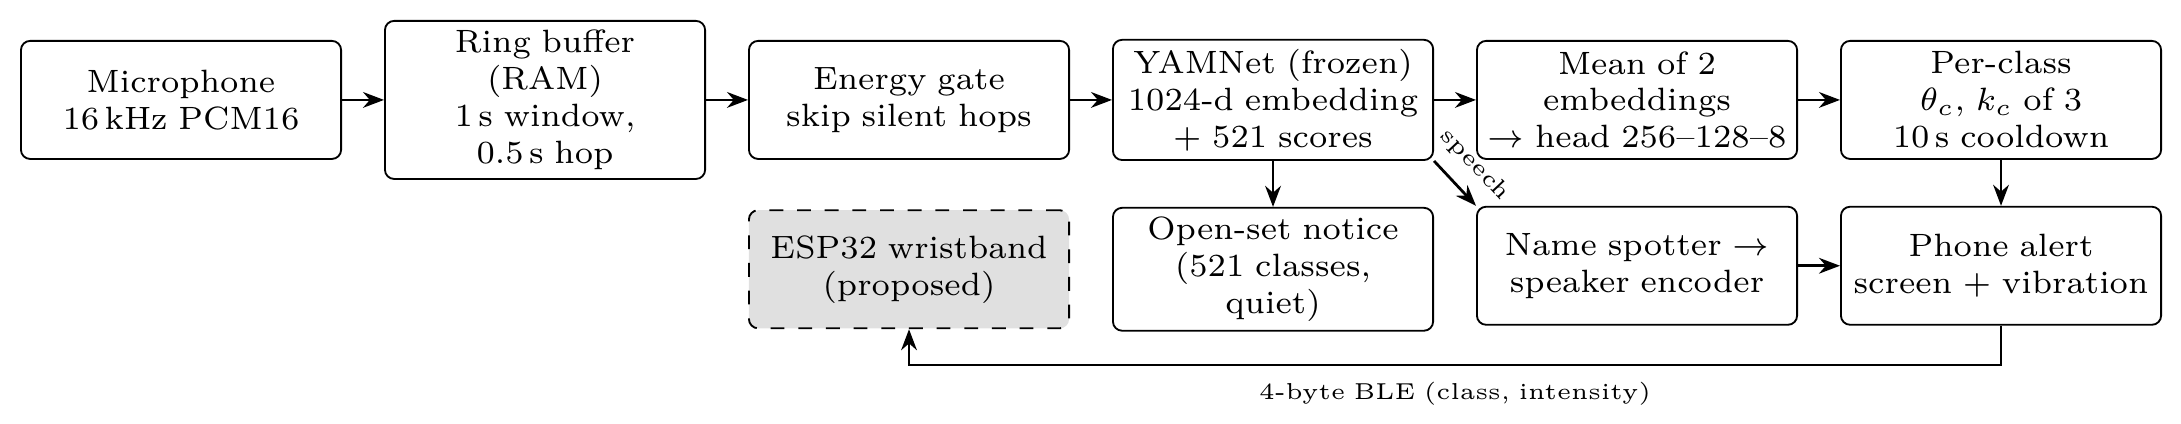
\includegraphics[width=\linewidth]{../assets/architecture.png}
\begin{itemize}
\item \textbf{On the phone:} 1\,s RAM buffer, energy gate, YAMNet embedding every 0.5\,s, head 256--128--8 (296k parameters).
\item \textbf{Alert rule:} per class, score $\ge\theta_c$ in $k_c$ of 3 windows, 10\,s cooldown.
\item \textbf{Budget tuning:} choose every $(\theta_c,k_c)$ on validation to maximise safety-weighted detection with $\le$ 4 false alarms/h in total.
\item \textbf{Data:} 22{,}549 clips from FSD50K, AudioSet, ESC-50, DESED + 329 SAHARA-IN; label IDs verified; splits grouped by recording.
\item \textbf{Name calls:} speech embeddings + head for ``Aryan''; GE2E speaker encoder names enrolled family, else ``Someone''.
\item \textbf{Home calibration:} record a sound 3 times; its threshold adapts, within a tested range.
\end{itemize}
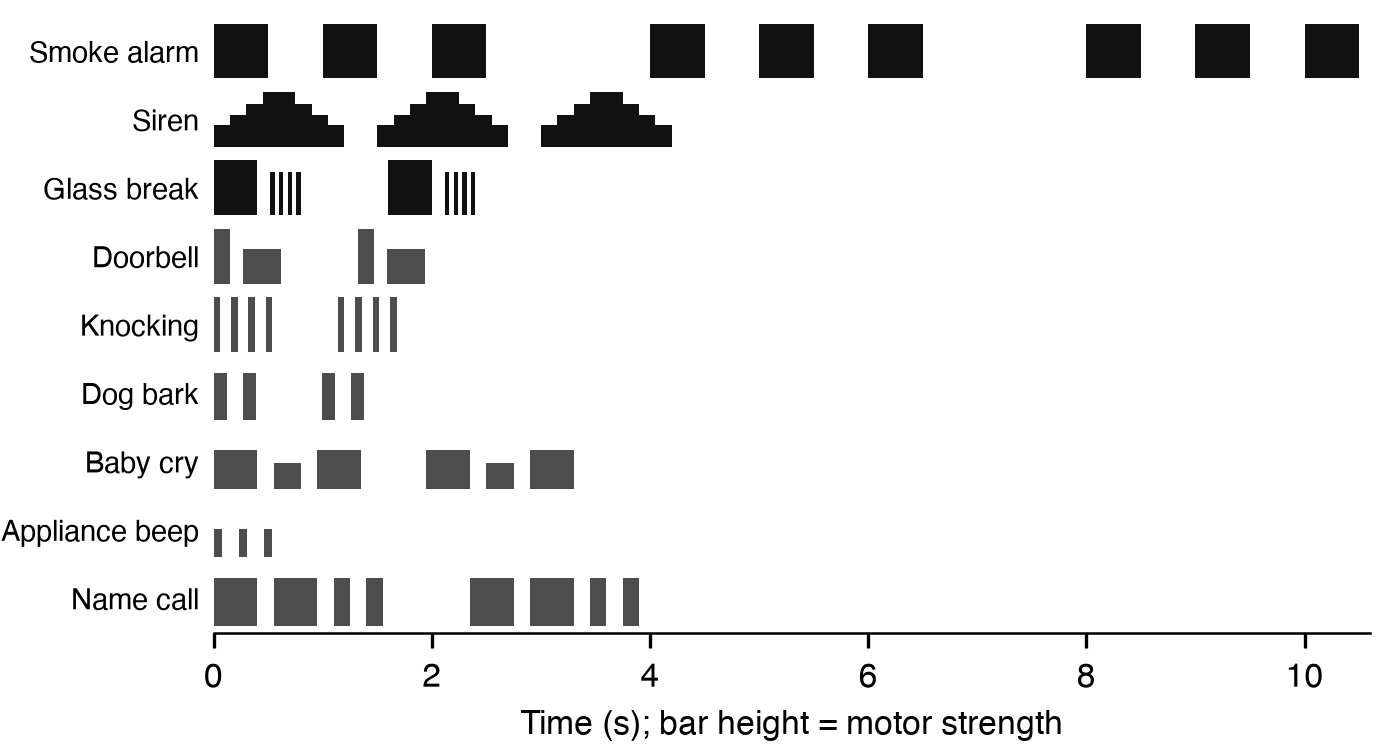
\includegraphics[width=0.85\linewidth]{../assets/haptics.png}\\
{\fontsize{15}{18}\selectfont Class-coded vibration patterns, same on phone and band.}
\end{psec}
\end{minipage}\hfill
\begin{minipage}[t]{0.25\linewidth}\vspace{0pt}
\begin{psec}{Results}
\textbf{Public test set:} \textbf{0.778 mAP}, macro F1 0.670, \textbf{3.5 false alarms/h} on 3.4\,h of continuous background.\\[2mm]
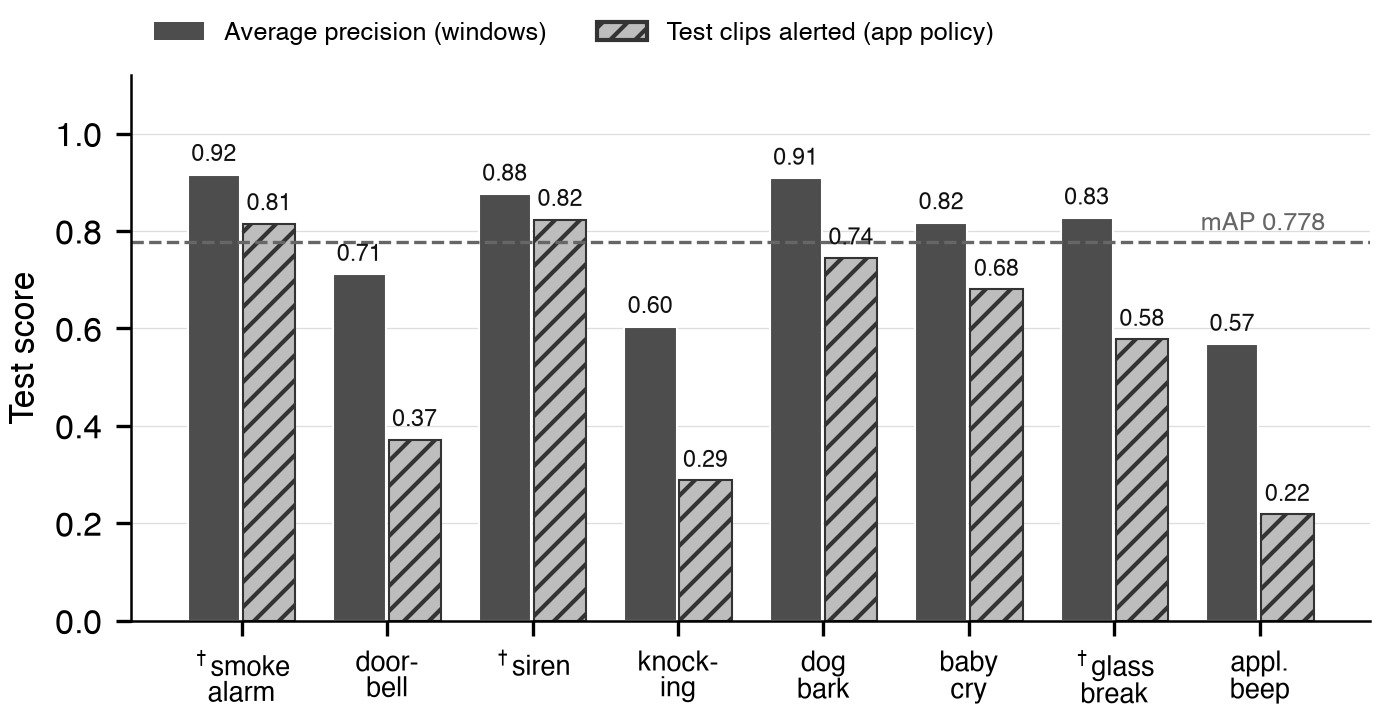
\includegraphics[width=0.9\linewidth]{../assets/test_ap.png}\\[2mm]
{\fontsize{17}{21}\selectfont
\begin{tabular}{@{}lrrr@{}}
\toprule
Alert rule (same model) & Clips & Safety & FA/h \\
\midrule
$\theta=0.5$, 1 window & 0.77 & 0.84 & 49.1 \\
$\theta=0.5$, 2 of 3 & 0.69 & 0.84 & 34.1 \\
\textbf{SAHARA tuned} & 0.54 & 0.69 & \textbf{6.1} \\
\bottomrule
\end{tabular}}\\[3mm]
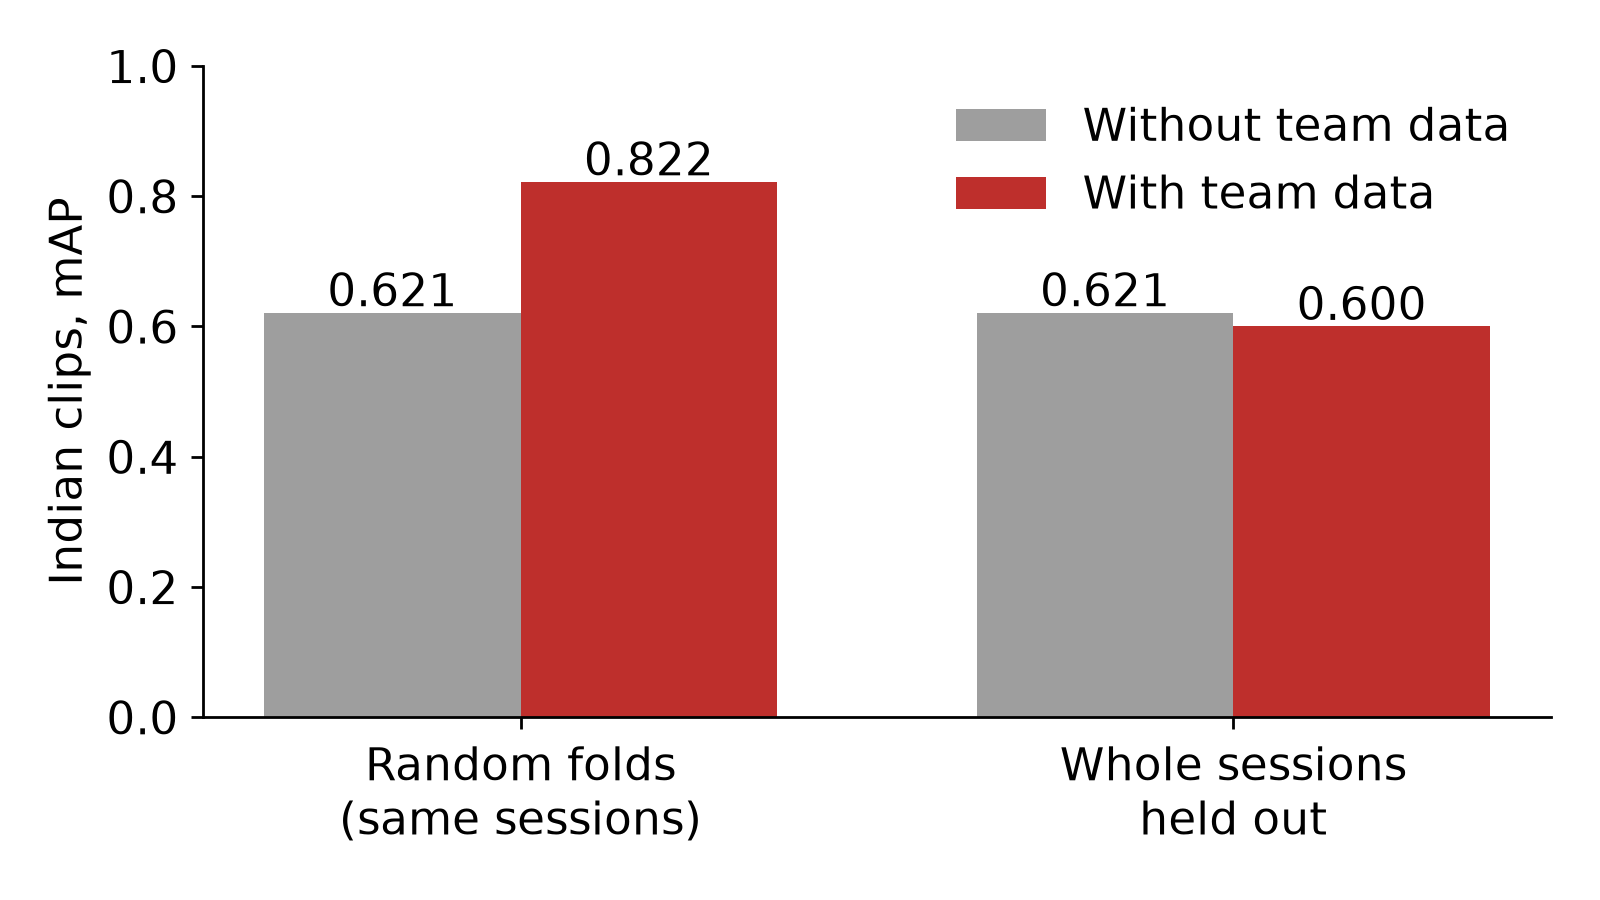
\includegraphics[width=0.49\linewidth]{../assets/indian_cv.png}\hfill
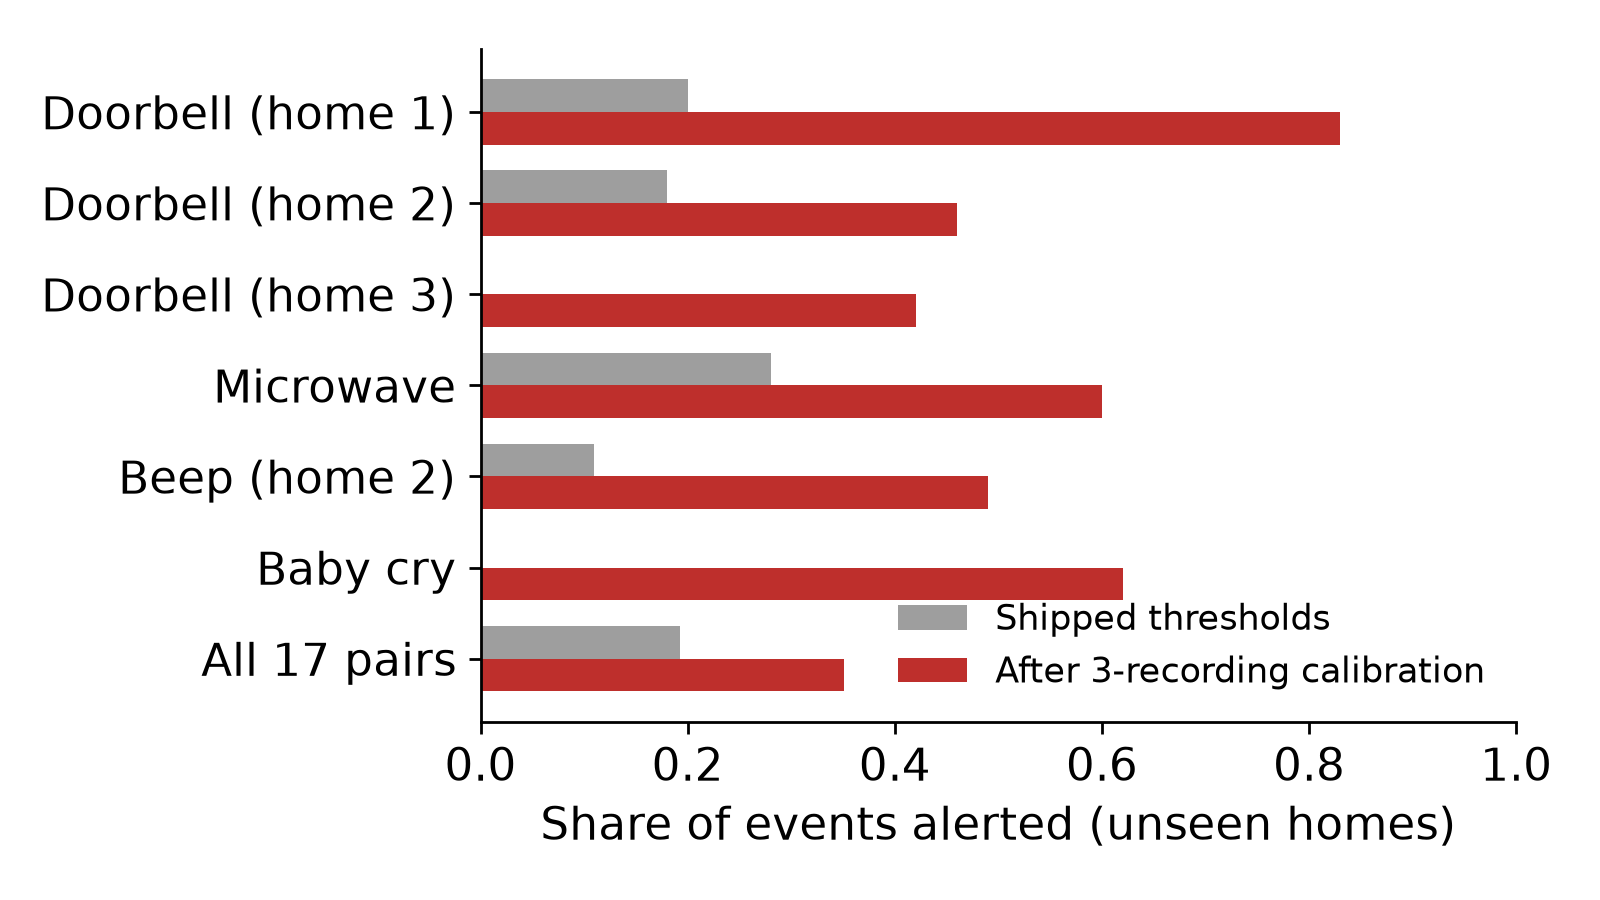
\includegraphics[width=0.49\linewidth]{../assets/calibration.png}\\[2mm]
{\fontsize{17}{21}\selectfont
\begin{tabular}{@{}lr@{}}
\toprule
Name call vs.\ background (AUC) & 0.872 \\
Name call vs.\ similar names (AUC) & 0.743 \\
Caller named correctly & 29/38 \\
Inference per window (Galaxy S24) & 20--29\,ms \\
\bottomrule
\end{tabular}}
\end{psec}
\end{minipage}\hfill
\begin{minipage}[t]{0.235\linewidth}\vspace{0pt}
\begin{psec}{Discussion}
\begin{itemize}
\item Budget tuning cut false alarms \textbf{34.1 $\rightarrow$ 6.1 per hour} on the same model.
\item Safety sounds are strongest: 22/27 smoke alarms, 28/34 sirens alerted.
\item Brief knocks and beeps are weakest.
\item Indian recordings help in homes the model has heard (0.62 $\rightarrow$ 0.82 mAP) but not yet in unseen homes (0.60).
\item \textbf{Home calibration} lifts unseen homes from 19\,\% to 35\,\% of events alerted, about +1 false alarm/h.
\item Wristband designed (\textasciitilde Rs.~870), firmware compiles; build and DHH user study are next.
\end{itemize}
\end{psec}

\begin{psec}{References}
{\fontsize{15}{18}\selectfont
\begin{enumerate}[leftmargin=8mm, itemsep=1pt, label={[\arabic*]}]
\item WHO, \textit{World Report on Hearing}, 2021.
\item MoHFW India, National Programme for Prevention and Control of Deafness.
\item D. Bragg et al., ASSETS 2016. \quad L. Findlater et al., CHI 2019.
\item D. Jain et al., HomeSound, CHI 2020; SoundWatch, ASSETS 2020; ProtoSound, CHI 2022.
\item J. Z. Huang et al., ``Not there yet'', ASSETS 2023.
\item J. F. Gemmeke et al., AudioSet, ICASSP 2017. \quad M. Plakal, D. Ellis, YAMNet, 2020.
\item E. Fonseca et al., FSD50K, IEEE/ACM TASLP 2022. \quad N. Turpault et al., DESED, DCASE 2019.
\item L. Wan et al., GE2E, ICASSP 2018. \quad C. Elkan, IJCAI 2001.
\end{enumerate}}
\end{psec}

\begin{psec}{Acknowledgements}
We thank our mentor \textbf{Prof.\ Priti Rumao} and the Department of Computer Engineering, MPSTME, for their guidance.
\end{psec}

\begin{tcolorbox}[colback=nmlight, colframe=nm, boxrule=1.2pt, arc=2mm, left=5mm, right=5mm]
{\fontsize{22}{27}\selectfont\bfseries\rmfamily\color{nm} Group}\\[1mm]
{\fontsize{18}{23}\selectfont
\begin{tabular}{@{}ll@{}}
Raj Singh & 70022300051 \\
Prachi Teotia & 70022300162 \\
Advika Mishra & 70022300146 \\
Mahi Mayani & 70022300180 \\
\end{tabular}\\[2mm]
\textbf{Mentor:} Prof.\ Priti Rumao}
\end{tcolorbox}
\end{minipage}
\end{document}
